\section{Krypto Hilfsskripte}

\begin{figure}[htbp] \label{fig:PCR_belegung}
    \centering
    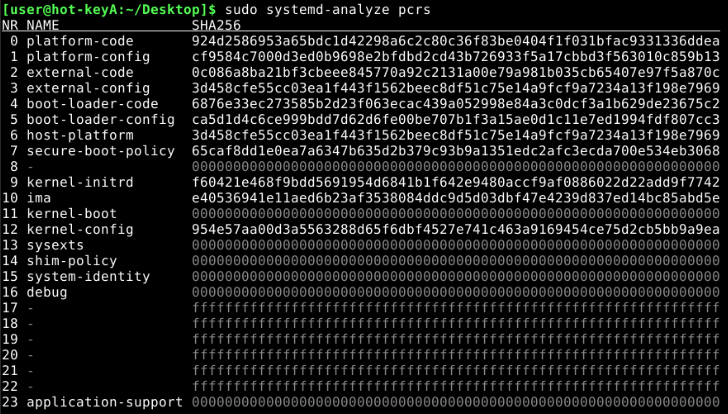
\includegraphics[width=0.8\textwidth]{Doku/Abbildungen/PCR_check.png}
    \caption{Log aus der \ac{PCR}-Abfrage. Quelle: Eigene Bildschirmaufnahme in NixOS.}
    \label{fig9:tpm_pcr}
\end{figure}


\begin{table}[htbp]
\centering
\footnotesize
\setlength{\tabcolsep}{4pt}
\renewcommand{\arraystretch}{1.2}
\begin{xltabular}{\linewidth}{@{} >{\ttfamily\RaggedRight}p{4.2cm} l >{\RaggedRight}X @{}}
\toprule
\textbf{\normalfont Skript} & \textbf{System} & \textbf{Zweck / Auslöser} \\
\midrule
\multicolumn{3}{@{}l}{\textit{Basis-System (Hot-Wallet, \path{scripts/ops/})}}\\
\addlinespace
refill/psbt\_export.sh    & Basis & Wartende Cold-\ac{PSBT} auf das Wechselmedium exportieren (Zustand COLD\_STARTED). \\
refill/psbt\_broadcast.sh & Basis & Signierte Cold-\ac{PSBT} vom Medium importieren, finalisieren und über Bitcoin Core broadcasten. \\
setup/wallet\_import.sh   & Basis & Cold-\path{wsh}-Deskriptor in Bitcoin Core und PostgreSQL registrieren. \\
setup/wgHMAC\_import.sh   & Basis & \ac{HMAC}-Geheimnis und WireGuard-Konfiguration vom Medium einspielen. \\
setup/wgPeer\_export.sh   & Basis & WireGuard-Peer-Konfiguration des Basis-Systems exportieren. \\
setup/wg\_setup.sh        & Basis & WireGuard-Interface und Kernel-Forwarding einrichten. \\
\addlinespace
\multicolumn{3}{@{}l}{\textit{Signierer-\ac{VM} (Key~A, Desktop)}}\\
\addlinespace
wgHMAC\_export.sh & Key~A & \ac{xpub}/öffentliche Deskriptoren, \ac{HMAC}-Geheimnis und WG-Konfiguration auf \ac{USB} exportieren. \\
wgPeer\_setup.sh  & Key~A & WireGuard-Peer einrichten bzw.\ überschreiben. \\
setup.sh          & Key~A & NixOS der Signierer-\ac{VM} automatisiert installieren. \\
mnt/umnt/format-USB.sh & Key~A & Wechselmedium mounten, sicher auswerfen bzw.\ bereinigen. \\
\addlinespace
\multicolumn{3}{@{}l}{\textit{Cold-\acp{VM} (Key~B/C, Desktop, \path{setup/})}}\\
\addlinespace
setup.sh          & Cold & NixOS-Cold-Image automatisiert installieren (LUKS, Flake-Pinning). \\
online.sh         & Cold & Kurzzeitig Online-Modus (specialisation) zur Wallet-Registrierung aktivieren. \\
airgap.sh         & Cold & In den air-gapped Standard zurückschalten. \\
mnt/umnt/format-USB.sh & Cold & Wechselmedium mounten, sicher auswerfen bzw.\ bereinigen. \\
\addlinespace
\multicolumn{3}{@{}l}{\textit{Evaluierte Hash-Freigabeschicht (verworfen, siehe \ref{sec:alt_hash})}}\\
\addlinespace
psbt/psbt-approve.sh   & Koord. & \ac{PSBT} hashen und Hash durch den Koordinator signieren (\path{unappr.<id>.psbt}). \\
auth/hash-keyGen.sh    & Koord. & Freigabe-Schlüsselpaar auf der Koordinator-Instanz erzeugen. \\
auth/hash-keyStore.sh  & Key~B/C & Public Key der Freigabe auf dem Signer hinterlegen (mit Air-Gap-Prüfung). \\
auth/hash-verify.sh    & Key~B/C & Freigabesignatur (\path{approval.json.sig}) vor dem Signieren verifizieren. \\
\bottomrule
\end{xltabular}
\caption{Betriebs- und Setup-Skripte je System.}
\label{tab:skripte}
\end{table}